%This is part of Un soupçon de mathématique sans être agressif pour autant
% Copyright (c) 2012-2013
%   Laurent Claessens
% See the file fdl-1.3.txt for copying conditions.

%+++++++++++++++++++++++++++++++++++++++++++++++++++++++++++++++++++++++++++++++++++++++++++++++++++++++++++++++++++++++++++ 
\section{Objectifs du chapitre}
%+++++++++++++++++++++++++++++++++++++++++++++++++++++++++++++++++++++++++++++++++++++++++++++++++++++++++++++++++++++++++++

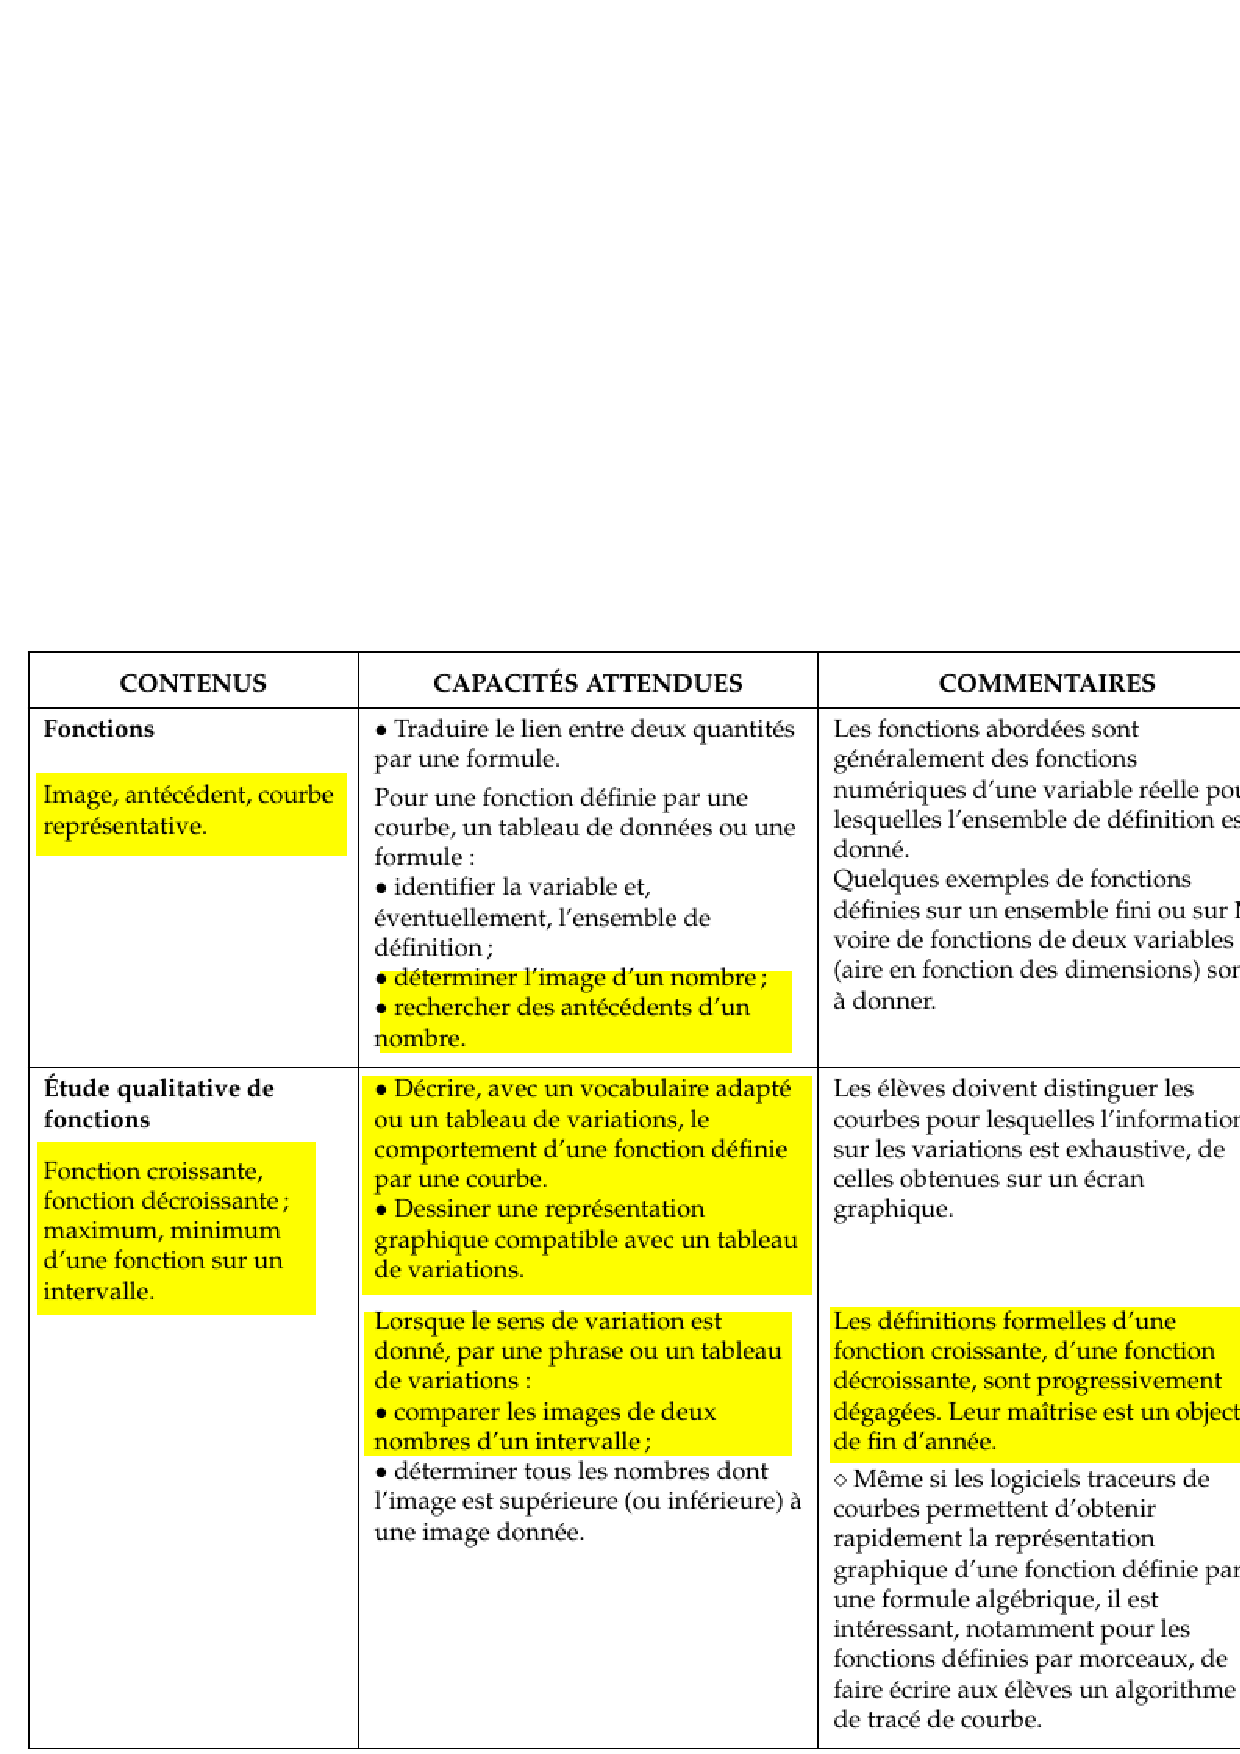
\includegraphics[width=\linewidth]{BO_fonctions_graphique.png}

%+++++++++++++++++++++++++++++++++++++++++++++++++++++++++++++++++++++++++++++++++++++++++++++++++++++++++++++++++++++++++++
\section{Courbe représentative d'une fonction}
%+++++++++++++++++++++++++++++++++++++++++++++++++++++++++++++++++++++++++++++++++++++++++++++++++++++++++++++++++++++++++++

% Partie graphique du berger syldave.
\begin{Aprojeter}
    %This is part of Un soupçon de mathématique sans être agressif pour autant
% Copyright (c) 2012-2013
%   Laurent Claessens
% See the file fdl-1.3.txt for copying conditions.

    Un berger syldave s'entraine pour le championnat national du lancer de chèvre. L'épreuve consiste à lancer une chèvre vers le haut depuis le bord d'une falaise située au bord d'un lac tranquille. La hauteur de la chèvre en fonction du temps par rapport à la surface du lac tranquille est une fonction \( f\) donnée par le graphique suivant.

    \begin{center}
        \input{Fig_WRXbDCo.pstricks}
    \end{center}
    La dernière partie du graphique correspond à la chèvre que l'on remonte rapidement hors de l'eau.
    À partir du graphique :
    \begin{enumerate}
        \item
            À quelle hauteur se trouve la chèvre au moment du lancer ?
        \item
            Pendant combien de temps la chèvre reste à une hauteur supérieure à celle à laquelle elle a été lancée ?
        \item
            À quel moment la chèvre atteint-elle sa hauteur maximale ? Quelle est cette hauteur ?
        \item
            À quelle hauteur se trouve la chèvre après \( 2.5\) secondes de vol ?
        \item
            Résumer toutes ces informations en dressant le tableau de variation de la fonction \( f\).
    \end{enumerate}

\end{Aprojeter}

\begin{definition}
Soit $f$ une fonction définie sur un ensemble $\defD$.
    On appelle \defe{représentation graphique}{représentation graphique (d'une fonction)}, ou le \defe{graphe}{graphe} de $f$, l'ensemble des points $(x,y)$ tels que $x\in\defD$ et $y=f(x)$.

    Lorsque \( y=f(x)\), le nombre \( y\) est l'\defe{image}{image par une fonction} de \( x\) par la fonction \( f\) et \( x\) est \emph{un} \defe{antécédent}{antécédent} de \( y\).
\end{definition}

\begin{Aretenir}
    La règle d'or des graphiques : le point de coordonnées \( (a;b)\) est sur le graphique de la fonction \( f\) si et seulement si \( f(a)=b\).
\end{Aretenir}

\begin{multicols}{2}

À propos du graphe ci-contre :
\begin{enumerate}
    \item
        Quel est l'ensemble de définition de la fonction \( f\) ?
    \item
        Quelle est l'image de \( 1\) par \( f\) ?
    \item
        Donner un antécédent de \( 3\).
    \item
        Que vaut \( f(-3)\) ?
    \item
        Quels sont les antécédents de \( -1\) ?
    \item 
        Quel est le maximum de \( f\) sur \( \mathopen[ -2 , 1 \mathclose]\) ?
    \item
        Quel est le maximum de \( f\) sur \( \mathopen[ -2 , 2 \mathclose]\) ?
\end{enumerate}
    
    \columnbreak

\begin{center}
   \input{Fig_AHAbqhj.pstricks}
\end{center}

\end{multicols}


%+++++++++++++++++++++++++++++++++++++++++++++++++++++++++++++++++++++++++++++++++++++++++++++++++++++++++++++++++++++++++++ 
    \section{Minimum et maximum}
%+++++++++++++++++++++++++++++++++++++++++++++++++++++++++++++++++++++++++++++++++++++++++++++++++++++++++++++++++++++++++++


Les notions de minima et maxima parlent, comme l'indiquent leurs noms en français, des points du graphe d'une fonction les plus hauts et les plus bas.

\begin{definition}
      Soit $f$ une fonction définie sur un intervalle \( I\).
      \begin{itemize}
            \item 
                Nous disons que le réel \( M\) est le \defe{maximum}{maximum} de \( f\) sur $I$ si et seulement si 
                \begin{enumerate}
                    \item
                        il existe $ a\in I$ tel que $f(a)=M$,
                    \item
                        \( f(x)\leq M\) pour tout $x\in I$.
                \end{enumerate}
                
          \item 
                Nous disons que le réel \( m\) est le \defe{minimum}{minimum} de \( f\) sur $I$ si et seulement si
                \begin{enumerate}
                    \item
                        il existe $ b\in I$ tel que $f(b)=m$,
                    \item
                        $f(x)\geq m$ pour tout \( x\in I\).
                \end{enumerate}
      \end{itemize}
\end{definition}

\begin{wrapfigure}[9]{r}{7.0cm}
   \vspace{-0.5cm}        % à adapter.
   \centering
   \input{Fig_MinMaxKNRdOd.pstricks}
\end{wrapfigure}

\begin{remark}
    Attention à deux choses.
    \begin{enumerate}
        \item
            Le minimum est la \emph{valeur} la plus basse, et non l'abscisse correspondante. Idem pour le maximum. 
        \item
            La minimum dépend de l'intervalle sur lequel on regarde la fonction.
    \end{enumerate}
\end{remark}

Une illustration sur la figure ci-contre. La fonction prend son maximum en \( x=a\) et ce maximum vaut \( M\). La fonction prend son minimum en \( x=b\) et ce minimum vaut \( m\).
